Because the relations between objects are essential for understanding the operator architecture, the following chapter should provide a more detailed description of how the objects interact and where there is loose and tight coupling.
For this reason, there is a diagram below showing the layout of the objects and their relations.


\begin{figure}[H]
	\centering
	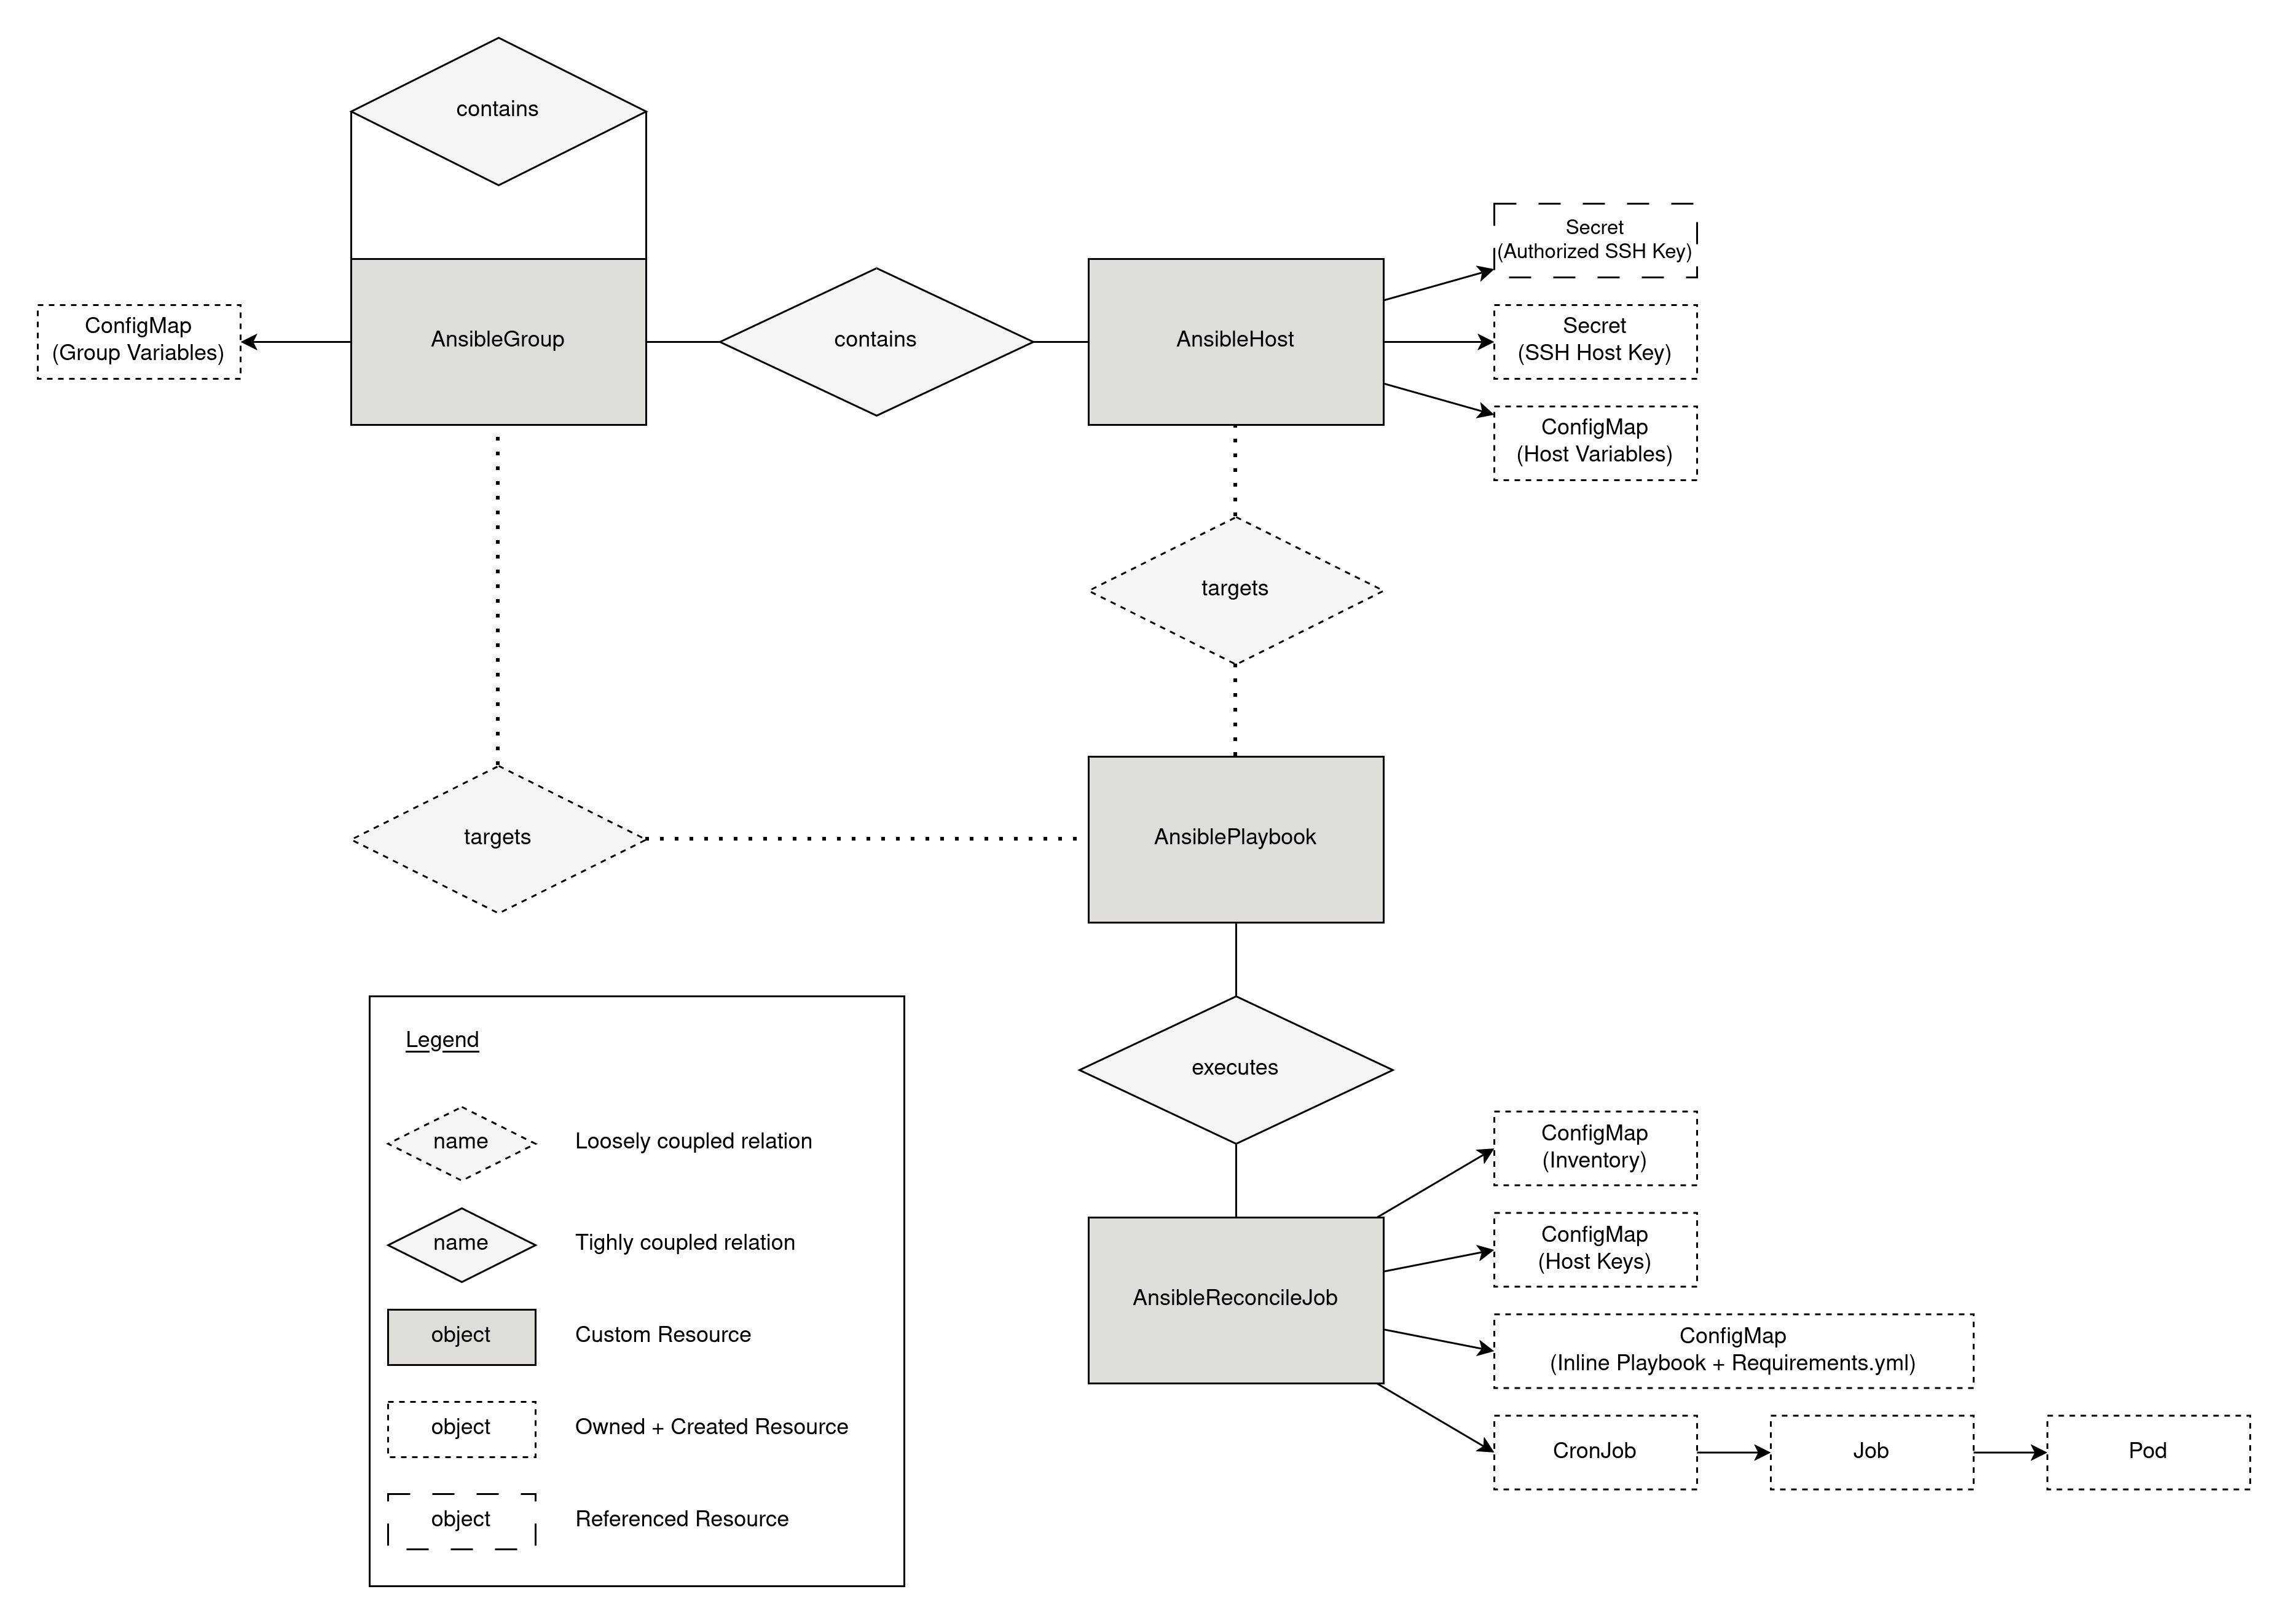
\includegraphics[width=1.1\textwidth]{bilder/object_relations.png}
	\caption{Object relations in the Operator}
	\label{pic:object_relations}
	\source{Own diagram}
\end{figure}

The graphic uses a notation adjacent to the classic Peter-Chen notation to show the relations.
As one can notice, the most relevant objects are created by the \anrecjob.

Several resources the operator manages need to contact external data sources or contact other external services in order to obtain their data or transfer information.
The diagram below shows the relations of resources inside the cluster to external resources.

\begin{figure}[H]
	\centering
	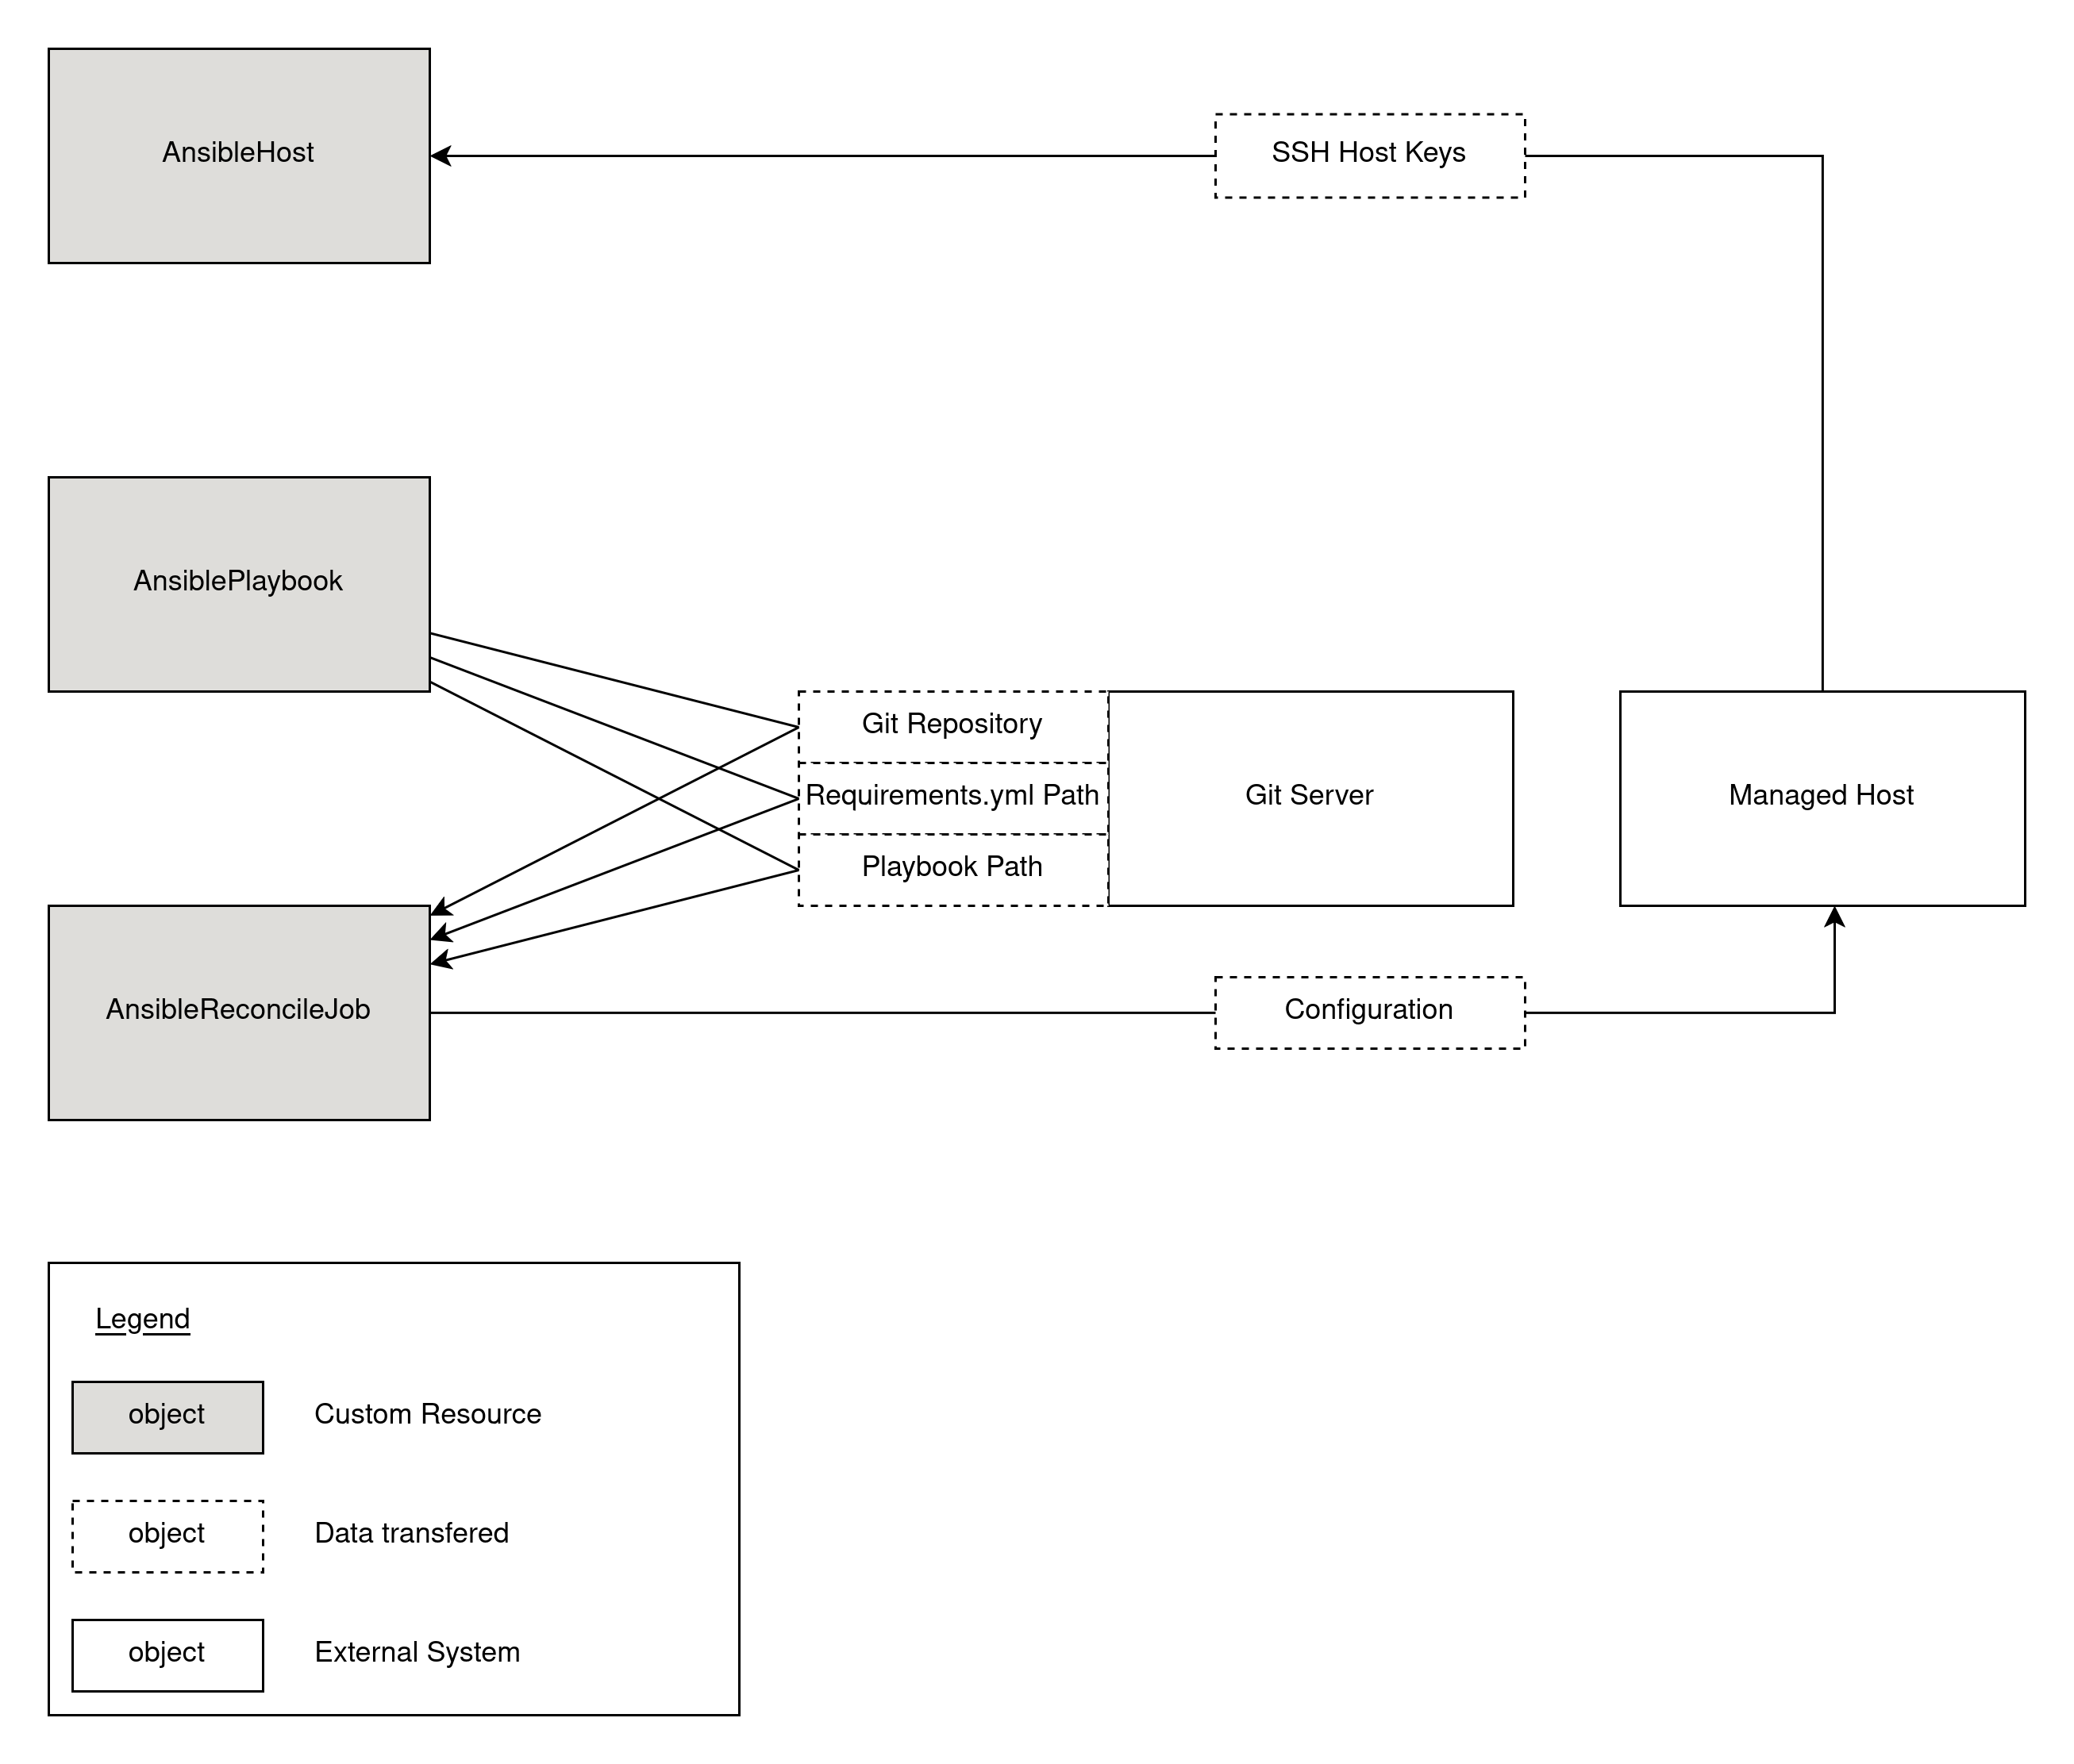
\includegraphics[width=1.1\textwidth]{bilder/Bachelor Thesis External Relations.drawio.png}
	\caption{Object relations to external data}
	\label{pic:object_data}
	\source{Own diagram}
\end{figure}
